\documentclass[a4paper,10pt]{article}
\usepackage[utf8]{inputenc}
\usepackage{hyperref}
\usepackage{graphicx}
%opening
\title{Le Protocole MQTT}
\author{Nicolas Vadkerti}
\usepackage{listings} % Required for inserting code snippets
\usepackage[usenames,dvipsnames]{color} % Required for specifying custom colors and referring to colors by name

\definecolor{DarkGreen}{rgb}{0.0,0.4,0.0} % Comment color
\definecolor{highlight}{RGB}{255,251,204} % Code highlight color

\lstdefinestyle{Style1}{ % Define a style for your code snippet, multiple definitions can be made if, for example, you wish to insert multiple code snippets using different programming languages into one document
language=Perl, % Detects keywords, comments, strings, functions, etc for the language specified
backgroundcolor=\color{highlight}, % Set the background color for the snippet - useful for highlighting
basicstyle=\footnotesize\ttfamily, % The default font size and style of the code
breakatwhitespace=false, % If true, only allows line breaks at white space
breaklines=true, % Automatic line breaking (prevents code from protruding outside the box)
captionpos=b, % Sets the caption position: b for bottom; t for top
commentstyle=\usefont{T1}{pcr}{m}{sl}\color{DarkGreen}, % Style of comments within the code - dark green courier font
deletekeywords={}, % If you want to delete any keywords from the current language separate them by commas
%escapeinside={\%}, % This allows you to escape to LaTeX using the character in the bracket
firstnumber=1, % Line numbers begin at line 1
frame=single, % Frame around the code box, value can be: none, leftline, topline, bottomline, lines, single, shadowbox
frameround=tttt, % Rounds the corners of the frame for the top left, top right, bottom left and bottom right positions
keywordstyle=\color{Blue}\bf, % Functions are bold and blue
morekeywords={}, % Add any functions no included by default here separated by commas
numbers=left, % Location of line numbers, can take the values of: none, left, right
numbersep=10pt, % Distance of line numbers from the code box
numberstyle=\tiny\color{Gray}, % Style used for line numbers
rulecolor=\color{black}, % Frame border color
showstringspaces=false, % Don't put marks in string spaces
showtabs=false, % Display tabs in the code as lines
stepnumber=5, % The step distance between line numbers, i.e. how often will lines be numbered
stringstyle=\color{Purple}, % Strings are purple
tabsize=2
}

\newcommand{\insertcode}[2]{\begin{itemize}\item[]\lstinputlisting[caption=#2,label=#1,style=Style1]{#1}\end{itemize}} 


% \insertcode{"Scripts/example.pl"}{Nena would be proud.} 

\begin{document}

\maketitle
\begin{abstract}
 

\url{https://github.com/SlaynPool/CR_MQTT/}\\
Le but de ce document est de concentrer une journée de recherche à propos du protocole MQTT. Pour tous lecteurs, je ne garantie en rien l'exactitude des informations present dans ce docuement.
 
 
\end{abstract}



\section{Presentation MQTT}
Comme vu en cours, MQTT est a la base dévelloppé pour permettre a des capteurs en plein millieu du dessert puissent remonter des données via des laisons sattellites. L'idée de MQTT etait donc d'avoir un protocole qui soit tolérant a la latence, économe en bande passante.\\
MQTT (Message Queuing Telemetry Transport) est donc très intéresant pour l'IOT. La légerté du protocole permet  l'implémenter sur quasiment n'importe quoi (L'exemple donné par oasis est un controlleur avec 256KB de Ram)\\
Le protocole MQTT a pour architecture un mode client serveur. Les clients sera nos Objets, et le serveur (communement appellé Broker) aura pour role de recevoir les informations envoyé par chacun de nos objets ainsi que de s'assurer que les informations demandé par les objets seront bien envoyés.

\subsection{Un client MQTT}
 Comme vu dans l'introduction, un client MQTT a pour objectif de soit envoyé des données, soit en recevoir. Pour cela, MQTT utilise un systeme de TOPIC. L'idée est donc d'avoir differents Topics sur le Broker, où l'on va pouvoir parlé avec notre objet, ecouter, ou faire les deux en meme temps.\\
 Pour mieux comprendre, on peut imaginer la situation suivante:\\
 On dispose d'objet qui sont capable de mesurer la temperatures et tous connecter au meme Broker MQTT.
 On decide d'une logique dans nos topics et ainsi:
 \begin{itemize}
  \item L'objet present sur le toit de l'IUT ecrira sur le topic /capteurs/temperatures/toit
  \item L'objet dans le hall, sur le topic /capteurs/temperatures/hall
 \end{itemize}
Maintenant, imaginon un systeme de Climatisation qui utilise nos capteurs pour réguler la temperatures. Pour qu'il puisse récuperrer les informations de nos capteurs, il lui suffira de s'abonner a nos topics. Dès que le topic sera mis a jour, il recevra le nouveau message.
Ici, on a que deux capteurs, et s'abonner un a un à ceux ci est concevable. Mais imaginons que nous avons 2000 capteurs, cela les beaucoup moins. MQTT etant pensé dans une optique de Scalabilité, il est possible de :
\begin{itemize}
 \item D'écrire sur des topics qui n'existe pas encore et il sera crée. (exemple: Je rajoute un capteur dans la BU, il pourra ecrire sans configuration sur le broker dans /capteurs/temperatures/bu
 \item S'abonner a des groupes de topics. Si on a aussi des capteurs de pression par exemple qui ecrive dans /capteurs/pression/lieux , on peut s'abonner a tous les topics qui parlent pression comme ceci : /capteurs/pression/+ ou si l'on veut tous les capteurs du hall, /capteurs/+/hall
 
\end{itemize}






\subsection{Le Broker}
Important: Le role du Broker n'est pas de stocker les données. On pourra utilisé une base de donné pour ceci. Cela n'est pas un problème. On peut considérer que le Broker ne sera pas une machine avec des capacités de calculs réduites contrairement a un Objets. Pour sauvegardé les mesages, il nous suffira d'avoir un client MQTT abonné a tous les topics qui remplira une BDD\\
Le rôle du Broker est de s'assurer de recevoir les messages publiés, ainsi que les transmettres aux abonnés. Pour cela, la notion de QoS est important pour déterminer sont comportement. 
\begin{itemize}
 \item Le message est envoyé avec pour QoS voulu 0\\
 Quand le broker recoit un message avec pour QoS 0, le mode par default, il ne doit renvoyé qu'une fois le message aux abonnés du topic. Il ne s'attend pas a recevoir d'accusé de récéption. On parle aussi de Best-Effort. On peut donc utilisé ce mode quand notre lien entre le client et le Broker est stable (Par exemple un cable ethernet)
 \item Le message est envoyé avec pour QoS voulu 1\\
 Le broker va envoyé le message tant que il n'aura pas recu d'accusé de récéption. Evidement, le probleme est que l'application doit etre programmé avec la possibilité de recevoir de fois le meme message, et donc etre capable de le détécter. Ce mode est a priviligié lorsque nous voulons etre sur de recevoir au moins une fois notre message. 
 \item Le message est envoyé avec pour QoS voulu 2
  C'est le mode qui s'assure que le destinataire recoit qu'une seul fois le message. L'expediteur du message va attendre en premier lieux un accusé de récéption, ce paquet lui indique qu'il peut detruire la donné qu'il a envoyé. Il envoie donc un message au receveur pour confirmé la destruction du paquet et l'emeteur fais de meme.
  \begin{figure}[h!]
\centering
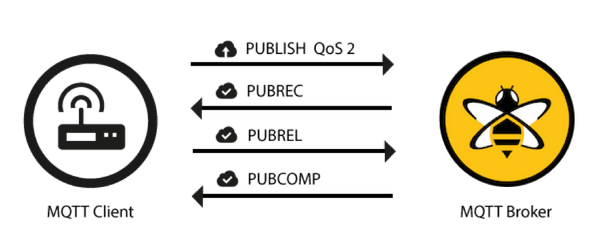
\includegraphics[scale=0.250]{qos.jpg}
\caption{QoS 3}
\label{fig:qos}
\end{figure}

Evidement, le soucis est que ce niveau de QoS est plus couteux, en temps, bande passante, etc ... Ce niveau de QoS est donc a utilisé lors de cas très particulier, où l'on ne peut pas ce permettre de a la fois perdre un paquet,  ou le reexpedier.

\end{itemize}

Nous n'en avons pas encore parler, cependant, il y a une notion de connection dans le protocole MQTT. En effet, un client, qui est abonné a un topic, mais qui n'est pas connecté va quand meme recevoir les messages noter avec pour QoS 1 et 2. Le Broker va bufferiser les messages a destination du client le temps qu'il soit connecté.


\section{Echange de trames Elementaires}

Pour cette partie, nous allons analyser quelques trames  communes du protocole MQTT. Le protocole MQTT est transporté grâce à TCP sur le port 1883.
 Voici tous d'abord la structure de toutes les trames MQTT

\begin{figure}[h!]
\centering
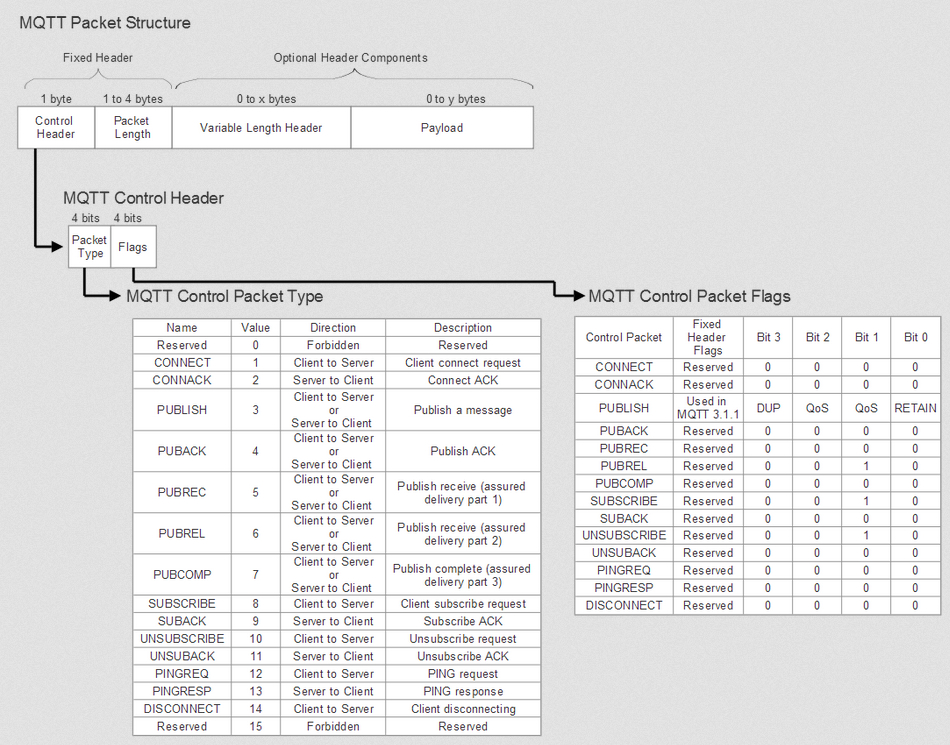
\includegraphics[scale=0.350]{paquet.jpg}
\caption{Un paquet MQTT}
\label{fig:paquet}
\end{figure}
Comme on peut le voir, seul les deux premiers parties d'un paquet sont obligatoire pour que MQTT.
\begin{itemize}
 \item La partie Control Header sur 1 octets qui a pour fonction d'annocer le but du paquet.\\
 \begin{itemize}
            \item Par exemple, l'on veut se connecter a un broker il  prendra la valeur 1, en binaire le champs type de paquet  sera :\\
                    |0001|
            \item Le flags sera donc |0000| pour signaler que c'est une tentative de connection.
 \end{itemize}
Le contenu du paquet sera donc |0001 0000| pour une tentative de connection.
Si on suit correctement le shema, le serveur va donc lui repondre par une trame CONNACK (acceptation de connection) |0010 0000|

\item Le champs Taille du paquet permet d'annoncer la taille du 
\end{itemize}





 \section{Sources}

\begin{itemize}
 \item \url{https://www.oasis-open.org/committees/tc_home.php?wg_abbrev=mqtt}
 \item \url{https://www.hivemq.com/blog/mqtt-essentials-part-6-mqtt-quality-of-service-levels/}
 \item \url{http://docs.oasis-open.org/mqtt/mqtt/v3.1.1/errata01/os/mqtt-v3.1.1-errata01-os-complete.html#_Toc442180841}
 \item \underline{Hands-On Internet of Things with MQTT} Author(s): Pulver, Tim Publisher: Packt Publishing Pub. Date: 2019
 \item \url{https://www.oreilly.com/library/view/internet-of-things/9781788470599/6078c828-0f58-4cdc-8275-fadb0eae40f4.xhtml}
\end{itemize}



\end{document}
